\subsection{CUG02 Iniciar Sesión Empleado}
\textsc{\begin{figure}[htbp!]
    \centering
        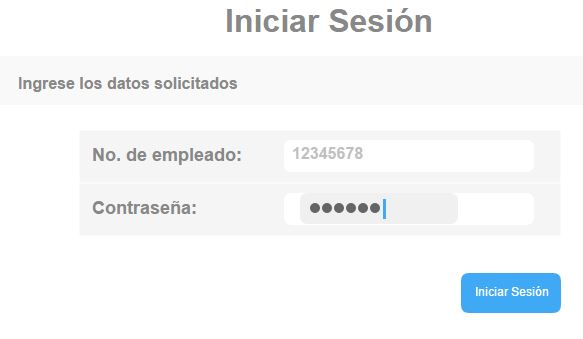
\includegraphics[width=0.7\textwidth]{images/UI/IniciarSesion/IniciarSesionA}
    \caption{UIIniciarSesión}
\end{figure}}

\textsc{\begin{figure}[htbp!]
    \centering
        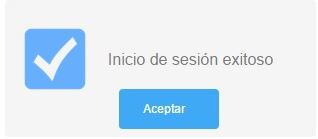
\includegraphics[width=0.5\textwidth]{images/UI/IniciarSesion/ACIS}
    \caption{AlertaConfirmaciónIniciarSesión}\end{figure}}

\textsc{\begin{figure}[htbp!]
    \centering
        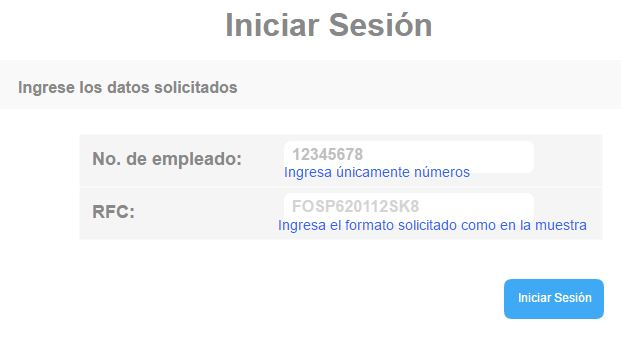
\includegraphics[width=0.5\textwidth]{images/UI/IniciarSesion/Mensaje2}
    \caption{MensajeFormatoIncorrecto}
\end{figure}}

\textsc{\begin{figure}[htbp!]
    \centering
        
\includegraphics[width=0.5\textwidth]{images/UI/IniciarSesion/alerta2}
    \caption{AlertaDatosIncorrectos}
\end{figure}}

\subsection{CUA02 Actualizar estado}

\textsc{\begin{figure}[htbp!]
    \centering
        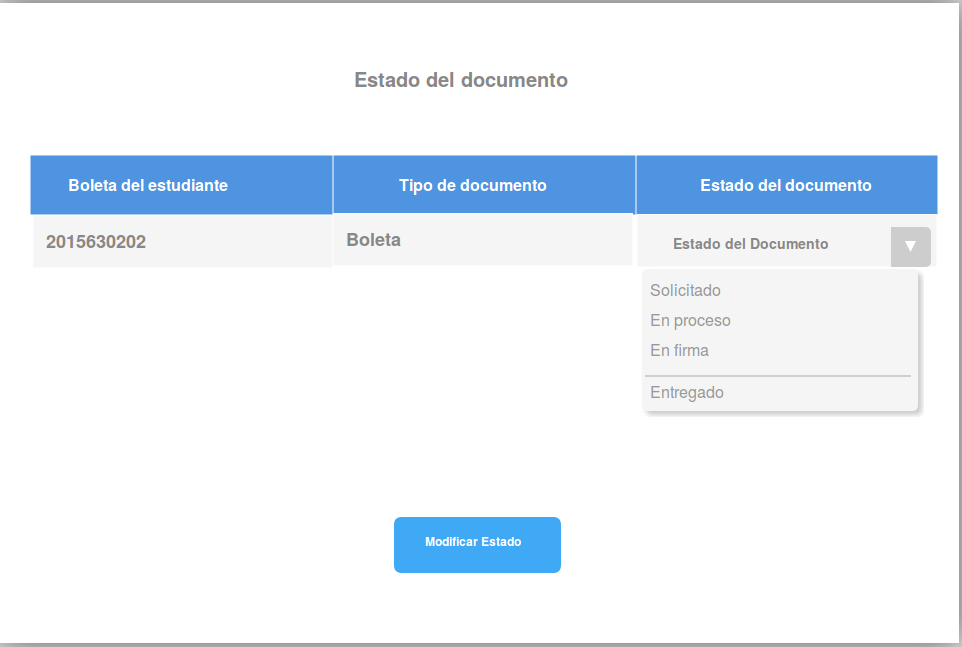
\includegraphics[width=0.5\textwidth]{images/UI/Analista/ActualizarEstado}
    \caption{ActualizarEstado}
\end{figure}}

\textsc{\begin{figure}[htbp!]
    \centering
        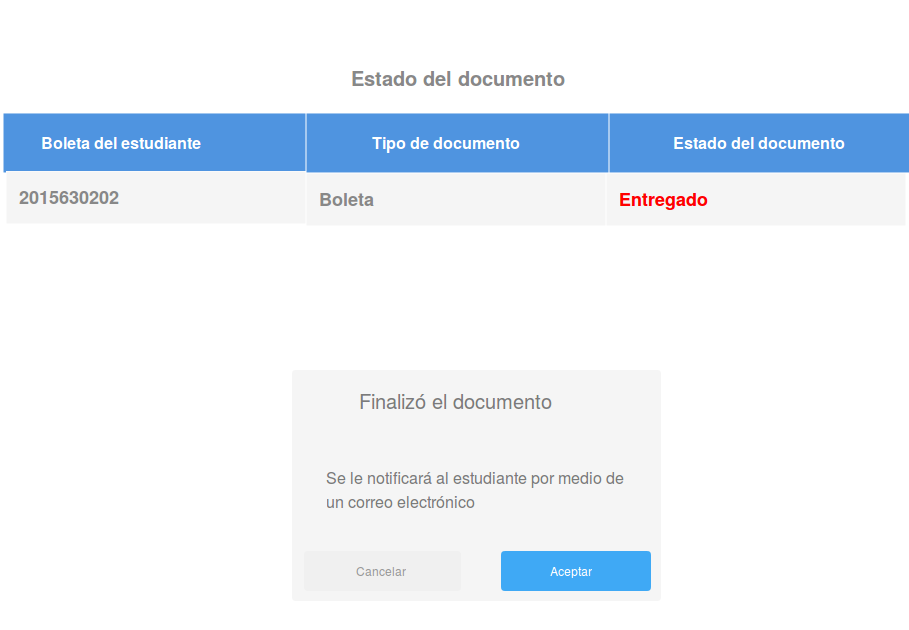
\includegraphics[width=0.5\textwidth]{images/UI/Analista/ActualizarEstadoA}
    \caption{AlertaActualizarEstado}
\end{figure}}


\textsc{\begin{figure}[htbp!]
    \centering
        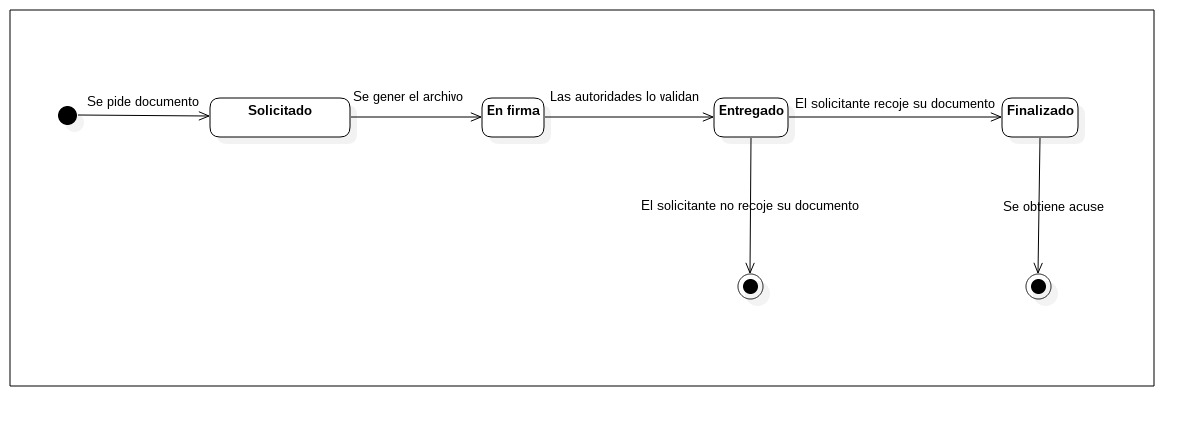
\includegraphics[width=0.5\textwidth]{images/UI/Analista/diagramEst}
    \caption{Diagrama de estados del documento}
\end{figure}}

\subsection{CUA03 Gestionar solicitudes}

\textsc{\begin{figure}[htbp!]
    \centering
        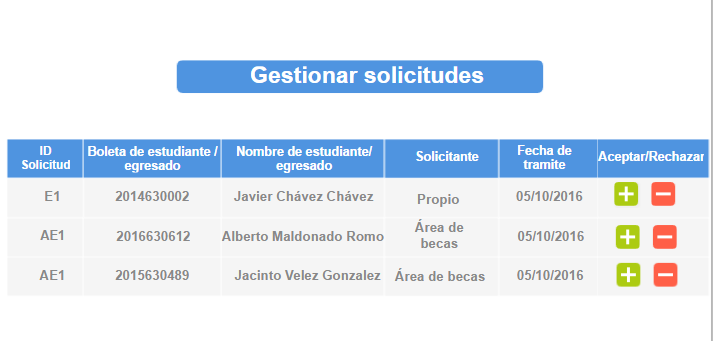
\includegraphics[width=0.7\textwidth]{images/UI/Analista/gestionarsolicitudes}
    \caption{Gestionar solicitudes}
\end{figure}}

\textsc{\begin{figure}[htbp!]
    \centering
        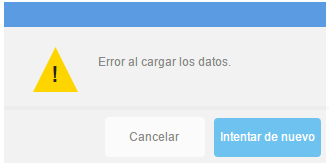
\includegraphics[width=0.5\textwidth]{images/UI/Analista/Errorconexion}
    \caption{Error cargar datos}
\end{figure}}

\textsc{\begin{figure}[htbp!]
    \centering
        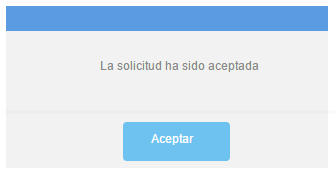
\includegraphics[width=0.5\textwidth]{images/UI/Analista/AlertaAceptado}
    \caption{AlertaAceptado}
\end{figure}}

\textsc{\begin{figure}[htbp!]
    \centering
        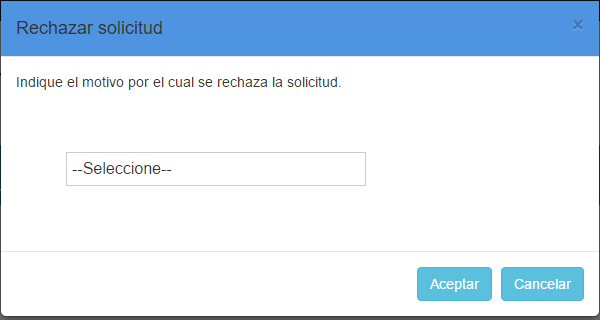
\includegraphics[width=0.5\textwidth]{images/UI/Analista/AlertaRechazar}
    \caption{AlertaRechazar}
\end{figure}}


